\documentclass{article}

\usepackage{graphicx}
\usepackage{tikz}
\usepackage{tikzsymbols}
\usetikzlibrary{calc,patterns,shapes.geometric}
\pagestyle{empty}
\usepackage[margin=0pt]{geometry}
\geometry{papersize={14in,12in}}

\def\centerarc[#1](#2)(#3:#4:#5){\draw[#1] ($(#2)+({#5*cos(#3)},{#5*sin(#3)})$) arc (#3:#4:#5);}

\begin{document}
	\begin{figure}
		\centering
		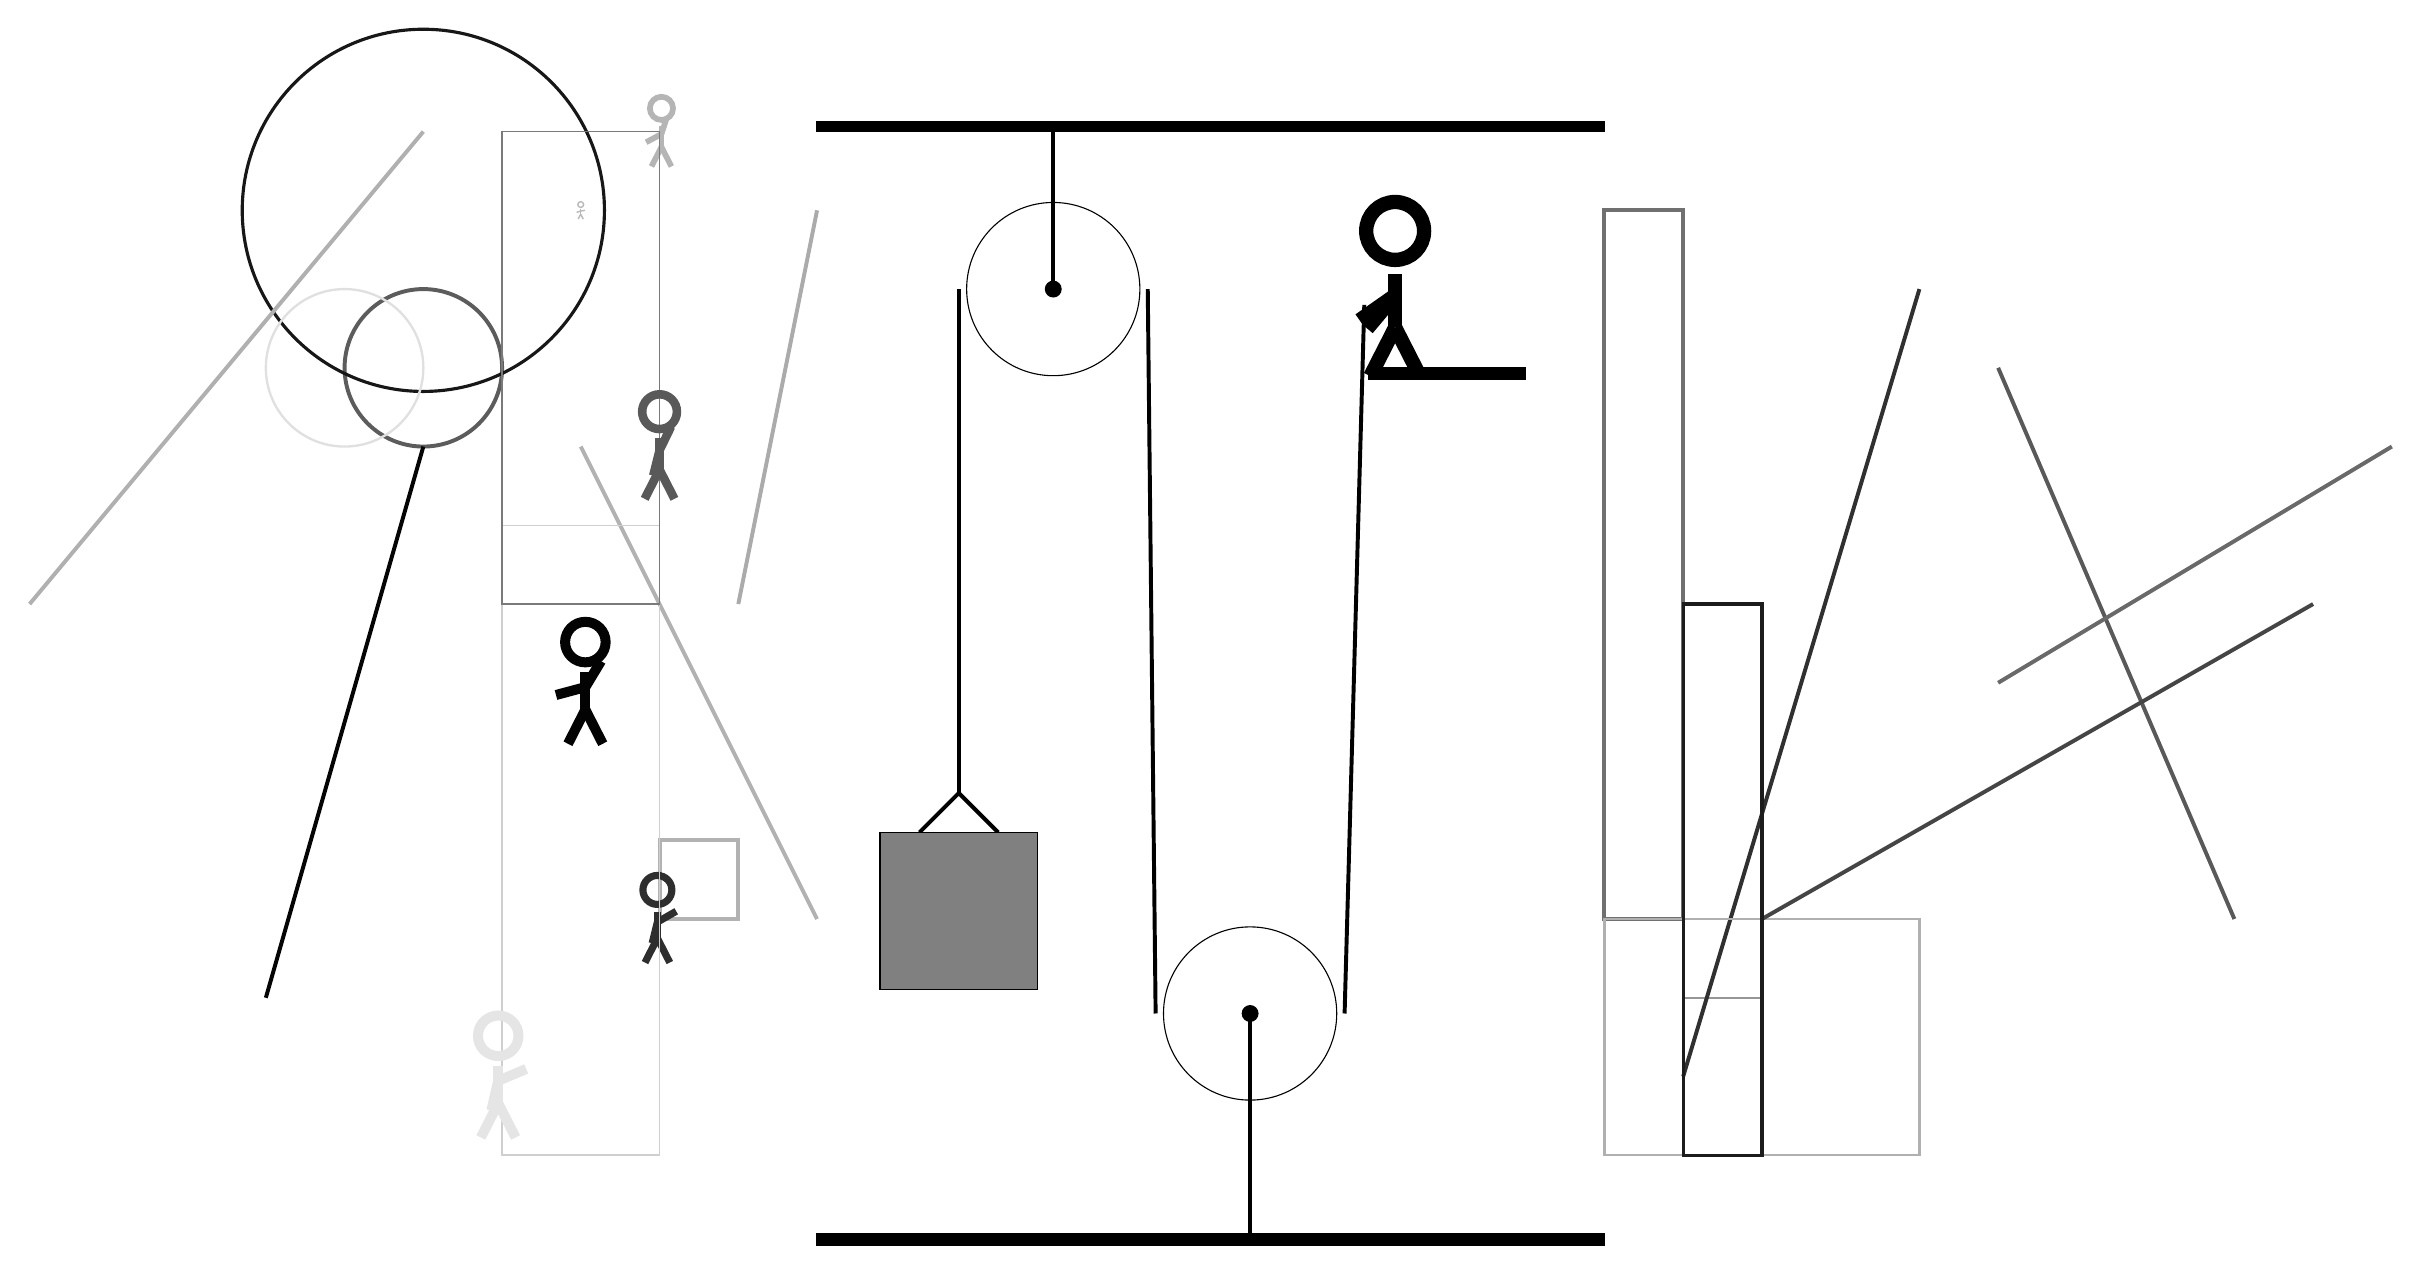
\begin{tikzpicture}
			%%%%% START %%%%%
			
			\draw[fill=black] (-2, 14) rectangle (8, 14.125);
			
			\node[line width=0.7mm, color=black!29] at (-4, 14) {\Strichmaxerl[4][28][72]};
			
			\node[line width=0.3mm, color=black!99] at (-5, 7) {\Strichmaxerl[7][15][59]};
			\draw[line width=0.5mm, color=black!65](13, 11) -- (16, 4);
			\draw[line width=0.2mm, color=black!41] (10, 8) rectangle (9, 3);
			
			\draw[line width=0.5mm, color=black!56] (9, 13) rectangle (8, 4);
			
			\draw [line width=0.5mm, color=black!64](-7, 11) circle (1.0);
			\draw[line width=0.5mm, color=black!30](-2, 4) -- (-5, 10);
			\draw[line width=0.5mm, color=black!81](9, 2) -- (12, 12);
			\draw[line width=0.5mm, color=black!30] (-3, 5) rectangle (-4, 4);
			\node[line width=0.2mm, color=black!27] at (-5, 13) {\Strichmaxerl[1][20][8]};
			\draw [line width=0.4mm, color=black!91](-7, 13) circle (2.3);
			
			\draw[line width=0.3mm, color=black!31] (8, 1) rectangle (12, 4);
			\draw[line width=0.5mm, color=black!31](-7, 14) -- (-12, 8);
			
			\node[line width=0.2mm, color=black!82] at (-4, 4) {\Strichmaxerl[5][76][30]};
			\draw[line width=0.2mm, color=black!19] (-4, 9) rectangle (-6, 1);
			\draw[line width=0.5mm, color=black!59](13, 7) -- (18, 10);
			
			\draw[line width=0.5mm, color=black!98](-7, 10) -- (-9, 3);
			
			\node[line width=0.7mm, color=black!10] at (-6, 2) {\Strichmaxerl[7][77][23]};
			\draw[line width=0.2mm, color=black!52] (-4, 8) rectangle (-6, 14);
			\draw[line width=0.5mm, color=black!93](9, 4) -- (9, 4);
			\draw[line width=0.5mm, color=black!33](-3, 8) -- (-2, 13);
			
			\draw [line width=0.3mm, color=black!12](-8, 11) circle (1.0);
			\draw[line width=0.5mm, color=black!73](10, 4) -- (17, 8);
			\node[line width=0.4mm, color=black!65] at (-4, 10) {\Strichmaxerl[6][76][64]};
			\draw[line width=0.4mm, color=black!89] (10, 8) rectangle (9, 1);
			
			
			\draw (3.5, 2.8) circle (1.1);
			\draw[fill=black] (3.5, 2.8) circle (0.1);
			\draw[line width=0.5mm] (3.5, 2.8) -- (3.5, 0);
			
			\draw (1, 12) circle (1.1);
			\draw[fill=black] (1, 12) circle (0.1);
			\draw[line width=0.5mm] (1, 14) -- (1, 12);
			
			\draw[line width=0.5mm](-0.7, 5.1) --  (-0.2, 5.6) -- (0.3, 5.1);
			\draw[fill=black!50] (-1.2, 5.1) rectangle (0.8, 3.1);
			
			\draw[line width=0.5mm](-0.2, 12) -- (-0.2, 5.6);
			\centerarc[line width=0.5mm](1, 12)(180:0:1.2000000000000002)
			\draw[line width=0.5mm](2.2, 12) -- (2.3, 2.8);
			\centerarc[line width=0.5mm](3.5, 2.8)(180:360:1.2000000000000002)
			\draw[line width=0.5mm](4.7, 2.8) -- (4.95, 11.8);
			
			\node at (5.3, 12) {\Strichmaxerl[10][35][-130]};
			\draw[fill=black] (5, 11) rectangle (7, 10.85);
			
			\draw[fill=black] (-2, 0) rectangle (8, -0.15);
			
			%%%%% END %%%%%
		\end{tikzpicture}
	\end{figure}	
\end{document}